\documentclass[11pt,a4paper]{scrartcl}
\usepackage[top=2cm,bottom=3cm,left=2cm,right=2cm]{geometry}
\usepackage{fontspec}
\usepackage{polyglossia}
    \setdefaultlanguage{english}
% \usepackage[utf8]{inputenc}
% \usepackage[T1]{fontenc}
% \usepackage[english]{babel}
\usepackage{lmodern}
\usepackage{fixcmex}
\usepackage{csquotes}
\usepackage{enumitem}
\usepackage{mathtools}
\usepackage{amssymb}
\usepackage{amsfonts}
\usepackage{bbold}
\usepackage{siunitx}
    \sisetup{range-units=single}
    \DeclareSIUnit{\stu}{stu}   % simulation time unit
    \DeclareSIUnit{\svu}{stu}   % simulation voltage unit
\usepackage{physics}
\usepackage{textcomp}
\usepackage{gensymb}
\usepackage{wasysym}
\usepackage[version=4]{mhchem}
\usepackage{array}
\usepackage{booktabs}
\usepackage{graphicx}
    \graphicspath{{./img/}}
\usepackage{caption}
\usepackage{subcaption}
\usepackage{tikz}
    \usetikzlibrary{calc,external}
    \tikzexternalize[prefix=extern/]
\tikzexternaldisable
\usepackage{circuitikz}
\usepackage{pgfplots}
    \pgfplotsset{%
        compat=1.16,
        table/search path={data},
    }
\usepackage{todonotes}
\usepackage[%
    colorlinks=true, linkcolor=blue,
    % hidelinks
]{hyperref}

\usepackage[%
    backend=biber,
    natbib=true,
    sorting=nyt,
    url=true,
    doi=true,
    isbn=false,
    maxbibnames=3,
    maxcitenames=2,
    date=year,
    style=alphabetic,
]{biblatex}
\addbibresource{literatur.bib}


% math mode version of r, l, c column types
\newcolumntype{R}{>{$}r<{$}}
\newcolumntype{L}{>{$}l<{$}}
\newcolumntype{C}{>{$}c<{$}}

\newcommand*{\figref}[1]{fig.~\ref{#1}}

\newcommand{\eg}{e.\,g.}
\newcommand{\ie}{i.\,e.}

\newcommand{\myvec}[1]{\ensuremath{\mathbf{#1}}}
\newcommand{\myten}[1]{\ensuremath{\mathbf{#1}}}


\titlehead{Ruhr-Universität Bochum, SS 2019}
\subject{Fortgeschrittenen-Praktikum Theorie}
\title{Numerical Simulation of Cardiac Tissue Electrophysiology}
\subtitle{}
\author{Jeremiah Lübke, 108015230366}
\date{\today}
\publishers{Advisor: Dr. Jürgen Dreher}


\begin{document}

\maketitle

\setcounter{tocdepth}{2}
\tableofcontents

\newpage

\section{Introduction}
The human heart is a fascinating apparatus, which does its work in a
constant and reliable fashion - usually without disruption - for the whole
of a persons life. To put things into perspective, the heart of an average
human being performs
\begin{center}
\begin{tabular}[t]{C R l}
            & 70    & (typical rest pulse per minute) \\
    \times  & 1440  & (minutes per day) \\
    \times  & 365   & (days per year) \\
    \times  & 80    & (estimated average human life time) \\
    \sim    & \mathbf{3\times10^9} & beats per life time,
\end{tabular}
\end{center}
while a typical car engine performs
\begin{center}
\begin{tabular}[t]{C R l}
            & \num{300000}  & (km drive during the cars life time) \\
    /       & 50    & (km/h, average speed) \\
    \times  & 60    & (minutes per hour) \\
    \times  & \num{2200}    & (revolutions per minute) \\
    \sim    & \mathbf{8\times10^8} & duty cycles per life time.
\end{tabular}
\end{center}

Investigating the hearts physical working principle poses an interesting
challenge with undoubtedly many relevant applications such as gaining a deeper
understanding of and developing more advanced treatments for often dangerous
arrhythmia.

The heart muscles basic functionality is rhythmically contracting itself
triggered by electrical signals, which are being conducted by the heart muscle
cells (the cardiomyocytes) themselves: the cardiac tissue combines the ability
to both perform mechanical work and conduct electrical signals.  This is very
remarkable, because usually these tasks are separately take care of by muscle
and neural cells, respectively.

Going a little more into detail: pacemaker cells (specialized cardiomyocytes)
in the SA-node rhythmically generate action potentials which travel at about
\SIrange{.05}{1}{\metre\per\second} to the AV-node and from there after a delay
at about \SIrange{2}{4}{\metre\per\second} through the His and ventricular
bundles and the Purkinje fibres, eventually reaching the intended tissue and
causing its contraction.


\subsection{Structure of the Cardiomyocytes}
For a better understanding it is helpful to take a closer look at the
microscopic structure of the cardiomyocytes:

Cardiomyocytes are tubular cells, which are enclosed by the \emph{sarcolemma}
(a double lipid-layered membrane) and contain chains of \emph{myofibril}
(fibres composed of long proteins), which are responsible for contraction of
the muscle tissue.  Additionally the cells contain the \emph{sarcoplastic
reticulum}, which is a membrane-enclosed region, mainly for storing
\ce{Ca^{2+}} ions.

In longitudinal direction \emph{interlacing disks} join the cells together
and via the \emph{gap junctions} allow propagation of action potentials.
Because of these features the heart muscle forms a \emph{syncytium}, \ie~the
whole of the single cells behaves like a single coordinated unit.


\subsection{Modeling the membrane potential}
Now the interior and exterior (\ie~the intermediate space between
neighbouring cells) regions of a cells exhibit different concentrations of
various ion species (this imbalance is being maintained by specialized ion
pumps and gates in the cell membrane), which results in a voltage between
those regions: the membrane potential $V=\Phi_i-\Phi_e$, which in the rest
case is equal to some rest potential $V_{\mathrm{rest}}$.

If at some point the membrane potential is perturbed by a stimulus in such
a way that it exceeds some threshold, the ion channels rapidly open causing
the concentration difference of the ions between interior and exterior
cell regions to invert resulting in a large upswing of the membrane
potential. This process is called \emph{depolarization} and the peak of the
membrane potential is called \emph{action potential}.
After reaching this peak the gates close again and the pumps recreate the
prior concentration difference which causes the membrane potential to
return to the rest value (\emph{repolarization}).

Since the membrane posses a finite specific electric capacity $C\,
[\si{\farad\per\metre\squared}]$,
the membrane potential obeys the capacitor equation:
\begin{equation}
    I=C\,\dv{V}{t}=-\sum_{s}I_{s}
    \label{eq:cap}
\end{equation}
were the total membrane current density $I$ is the sum of all involved
species-specific current densities.
Therewith the dynamics of $V$ can be modeled by modeling the
membrane current densities $I_s$.

\begin{figure}[h!]
    \centering
    \begin{circuitikz}
    \draw                               (5, 0)
        to[short,o-,l=intracellular]    (5, 1)
        to[short]                       (1, 1)
        to[C=$C_m$]                     (1, 5.5)
        to[short]                       (5, 5.5)
        to[short,-o,l=extracellular]    (5, 6.5);

    \draw                               (3, 5.5)
        to[short,i=$I_{\mathrm{Na}}$]   (3, 4)
        to[vR=Na gate]                  (3, 2.5)
        to[V,v=$V_{\mathrm{Na}}$]       (3, 1);

    \draw                               (6, 5.5)
        to[short,i=$I_{\mathrm{K}}$]    (6, 4)
        to[vR=K gate]                   (6, 2.5)
        to[V,v=$V_{\mathrm{K}}$]        (6, 1);

    \draw                               (5, 5.5)
        to[short]                       (9, 5.5)
        to[short,i=$I_{\mathrm{Ca}}$]   (9, 4)
        to[vR=Ca gate]                  (9, 2.5)
        to[V,v=$V_{\mathrm{Ca}}$]       (9, 1)
        to[short]                       (5, 1);

\end{circuitikz}


% vim: set ff=unix tw=79 sw=4 ts=4 et ic ai :

    \caption{Electrical circuit representing the membrane structure}
    \label{fig:circut}
\end{figure}


\subsection{Developing a Continuum Description}
\label{sec:contdescr}
At a microscopic level the propagation of action potential is a discrete
process (from cell to cell). However looking at tissue at sufficiently large
scales, it can be viewed as continuous (\textrightarrow~\emph{functional
syncytium}). It is important to note the anisotropic nature of this process:
the tissue exhibits different conductivities in longitudinal and transversal
direction with respect to the myofibril.

\subsubsection{Bidomain model}
One formulates potentials $\Phi_i, \Phi_e$ and current densities $\myvec{J_i},
\myvec{J_e}$ for the intra- and extracellular regions.  It is important to
note, that formally all of these functions are defined on the whole domain.

To set them into relation, consider Possion's equation and Ohm's Law:
\begin{gather*}
    \myvec{E}=-\nabla\Phi,\quad \myvec{J}=\myten{G}\,\myvec{E} \\
    \implies \myvec{J_i}=-\myten{G_i}\,\nabla\Phi_i,\quad
    \myvec{J_e}=-\myten{G_e}\,\nabla\Phi_e
\end{gather*}
where \myvec{E} is the electrical field associated with the potential $\Phi$
and \myten{G} is the conductivity tensor accounting for the anisotropy.

Imposing conservation of current:
\begin{equation*}
    \nabla\cdot(\myvec{J_i}+\myvec{J_e})=0 \implies
    -\nabla\cdot\myvec{J_i}=\nabla\cdot\myvec{J_e}=I_m
\end{equation*}
(where $I_m$ is the transmembrane current density with units
\si{\ampere\per\metre\cubed}), and rewriting the capacitor equation
\eqref{eq:cap}:
\begin{equation*}
    I_m=\beta\left(C\,\dv{V}{t}+\sum_{s}I_{s}\right),\quad V=\Phi_i-\Phi_e
\end{equation*}
(where $\beta$ is a scaling constant with units \si{\per\metre}), one finds
after some calculations:
\begin{subequations}
\begin{align}
    \nabla\cdot\myten{G_i}(\nabla{V}+\nabla\Phi_e)
    &=\beta\left(C\,\dv{V}{t}+I_{\mathrm{ion}}\right)
    \label{eq:i}
    \\
    \nabla\cdot\left((\myten{G_i}+\myten{G_e})\,\nabla\Phi_e\right)
    &=-\nabla\cdot(\myten{G_i}\,\nabla{V})
    \label{eq:ii}
\end{align}
\end{subequations}

Now one has a system of two coupled PDEs with \eqref{eq:i} being parabolic
and \eqref{eq:ii} being elliptic, which is rather difficult to solve.

\subsubsection{Monodomain model}
In order to make matters more accessible, one makes the assumption that the
intra- and extracellular anisotropies are identical, \ie~the respective
conductivities are proportional:
\begin{gather}
    \myten{G_e}=\lambda\,\myten{G_i} \nonumber \\ \implies
    \dv{V}{t}=\nabla\cdot\myten{D}\,\nabla{V}-\frac{1}{C}\sum_{s}I_{s}
    \label{eq:divcap}
\end{gather}
(with the conductivity tensor $\myten{D}=\frac{1}{C\beta}\myten{G}$)
which reduces the problem to one parabolic PDE (a diffusion equation).

Now all that is left to do is to model the conductivity tensor \myten{D} to
represent the tissue at hand.
One way of doing this is to split this object
into components parallel and perpendicular to the direction of the
myofibril \myvec{f}, like so
\begin{equation*}
    \myten{D}=\myten{D_{\perp}}\,\mathbb{1}+(\myten{D_{\parallel}}
    -\myten{D_{\perp}})\,\myvec{f}\,\myvec{f^T}
\end{equation*}
where for typical cardiomyocytes one has the relation
$D_{\parallel}/D_{\perp}\sim2\ldots10$.

Another way is to neglect the anisotropies all together and write the
conductivity tensor as a scalar value: $\myten{D}\to\eta$. This is the
approach taken by the following investigations.

\vspace{\baselineskip}
\emph{Note}: Without external stimuli (enforced by von Neumann boundary
conditions) bi- and monodomain models yield almost identical results.
However when considering such external stimuli (\eg~defibrillation) the
unequal anisotropies of intra- and extracellular regions are significant.


% vim: set ff=unix tw=79 sw=4 ts=4 et ic ai :


\newcommand{\Vtilde}{\ensuremath{\tilde{V}}}

\section{Three Models}
In this section I am going to describe three approaches -- out of an
abundance of available models (\url{www.cellml.org}) -- which can be used to
describe the dynamics of the membrane potential.

\subsection{Hudgkin \& Huxley (1952)}
This model was developed by A.~L.~Hodgkin and A.~F.~Huxley to fit
measurements taken on a giant squid axon prior to detailed knowledge about
the biophysical mechanisms being available.

The membrane current density is modeled as the sum of Sodium, Potassium and
a leakage current, each obeying Ohm's Law:
\begin{gather}
    I_m = \sum_{s}I_{s}=I_{\mathrm{Na}}+I_{\mathrm{K}}+I_{\mathrm{leak}} \\
    I_s = g_s\,(V-V_s) \nonumber
\end{gather}
where the specific conductivites are described by dimensionless gating
variables $n, m, h\in[0,1]$:
\begin{equation*}
    g_{\mathrm{Na}}=\bar{g}_{\mathrm{Na}}\,n^4,\quad
    g_{\mathrm{K}}=\bar{g}_{\mathrm{K}}\,m^3\,h,\quad
    g_{\mathrm{leak}}=\bar{g}_{\mathrm{leak}}
\end{equation*}

The respective rest potentials and maximal specific conductivities were measured as:
\begin{table}[h!]
    \centering
    \begin{tabular}{c | C C}
        \toprule
        Current & V_s/\si{\milli\volt} &
        \bar{g}_s/\si{\milli\siemens\per\centi\metre\squared} \\
        \midrule
        Na      & 115   & 120   \\
        K       & -12   & 36    \\
        leak    & 10    & 0.3   \\
        \bottomrule
    \end{tabular}
\end{table}

The gating variables obey the following ODEs:
\begin{subequations}
\begin{align}
    \dv{n}{t}&=\alpha_{n}\,(1-n)-\beta_{n} \label{eq:n} \\
    \dv{m}{t}&=\alpha_{m}\,(1-m)-\beta_{m} \label{eq:m} \\
    \dv{h}{t}&=\alpha_{h}\,(1-h)-\beta_{h} \label{eq:h}
\end{align}
\end{subequations}
with ($\Vtilde=V/\si{\milli\volt}$):
\begin{align*}
    \alpha_{n}&=\SI{.01}{\per\milli\second}
        \frac{\Vtilde-10}{1-
            \exp\left(\frac{10-\Vtilde}{10}\right)},&
    \beta_{n}&=\SI{.125}{\per\milli\second}
        \exp\left(-\frac{\Vtilde}{80}\right) \\
    \alpha_{m}&=\SI{.1}{\per\milli\second}
        \frac{\Vtilde-25}{1-
            \exp\left(\frac{25-\Vtilde}{10}\right)},&
    \beta_{m}&=\SI{4}{\per\milli\second}
        \exp\left(-\frac{\Vtilde}{18}\right) \\
    \alpha_{h}&=\SI{.07}{\per\milli\second}
        \exp\left(-\frac{\Vtilde}{20}\right),&
    \beta_{h}&=\frac{1}{1+
        \exp\left(\frac{30-\Vtilde}{10}\right)}
\end{align*}

Thus, one has to solve a system of four first-order uncoupled ODEs
(\ref{eq:cap}, \ref{eq:n}, \ref{eq:m}, \ref{eq:h}).


\subsection{Aliev \& Panfilov (1996)}


\subsection{Fenton et al (2002)}


% vim: set ff=unix tw=79 sw=4 ts=4 et ic ai :


\section{Dynamics of a Single Cell}
In this section the results of the numerical solutions for a single cell
using the three models presented above are discussed. All results were
obtained with a simple Forward-Euler scheme.


\subsection{Hodgkin \& Huxley}
The equations were integrated for \SI{10}{\milli\second} with a time step
$\Delta{t}=\SI{.01}{\milli\second}$ (\ie~1000 integrations steps) and an
initial potential $V_0=\SI{-7}{\milli\volt}$. The resulting action potential,
current densities and gating variables are plotted in \figref{fig:hh1}.

\begin{figure}[h]
    \centering
    \begin{subfigure}[h]{.3\textwidth}
        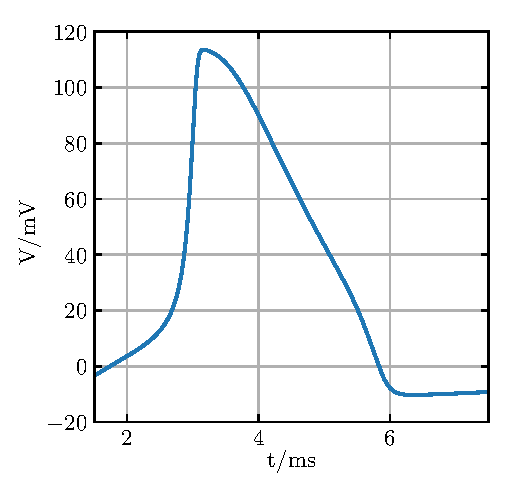
\includegraphics[width=\textwidth]{hh52-10ms-V}
        \vspace{-\baselineskip}
        \caption{Potential}
        \label{fig:hh1V}
    \end{subfigure}
    \begin{subfigure}[h]{.3\textwidth}
        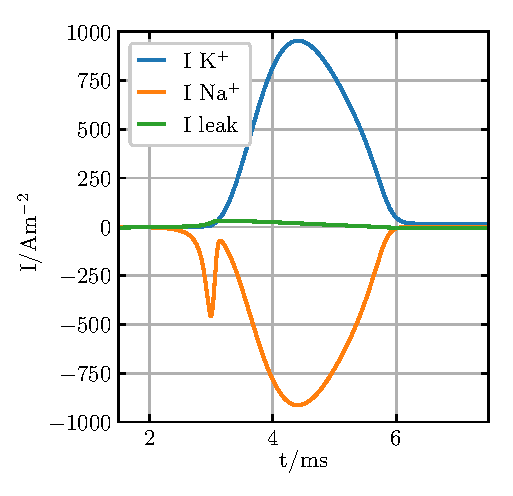
\includegraphics[width=\textwidth]{hh52-10ms-I}
        \vspace{-\baselineskip}
        \caption{Current Densities}
        \label{fig:hh1I}
    \end{subfigure}
    \begin{subfigure}[h]{.3\textwidth}
        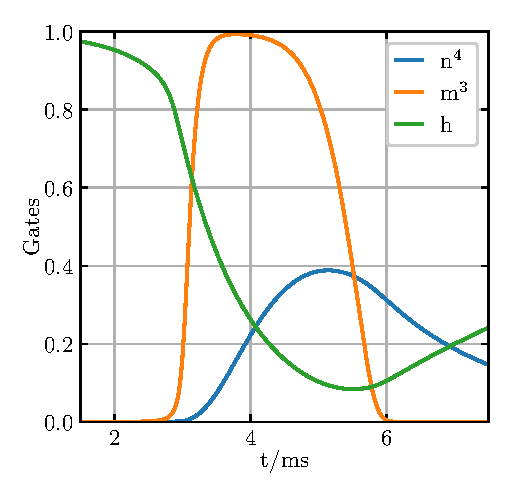
\includegraphics[width=\textwidth]{hh52-10ms-Gates}
        \vspace{-\baselineskip}
        \caption{Gating Variables}
        \label{fig:hh1Gates}
    \end{subfigure}
    \caption{Results of integrating the H\&H model}
    \label{fig:hh1}
\end{figure}

The gating variables were initially all set to 0, yet at
$t=\SI{0}{\milli\second}$ the \ce{Na+} gate $h$ jumps directly to being almost
completely open ($h(t=0)=0.99$); however, the \ce{Na+} current is at this point
suppressed by the closed $m$ gate. The $h$ gate slowly closes up to
$t\approx\SI{5}{\milli\second}$ and then swings down more rapidly, while at the same
time the $m$ gate opens strongly and allows for influx of \ce{Na+} ions
(interestingly the \ce{Na+} current exhibits a small seperate peak at
$t\approx\SI{5}{\milli\second}$ before rising up to its full strength). This
causes the membrane potential to rise up and become strongly positive. Shortly
after the quick opening of the $m$ gate, the \ce{K+} gate $n$ also opens,
allowing for an opposed \ce{K+} outflux causing the membrane potential to
eventually repolarize.

The resulting action potential resembles qualitatively the results depicted in
fig.~12 in \cite{HH52}. An even better fit is achieved when integrating the
system for \SI{40}{\milli\second} with and initial value of
$V_0=\SI{-30}{\milli\volt}$, as depicted in fig.~22 in \cite{HH52} (see
\figref{fig:hh2}).

\begin{figure}[h]
    \centering
    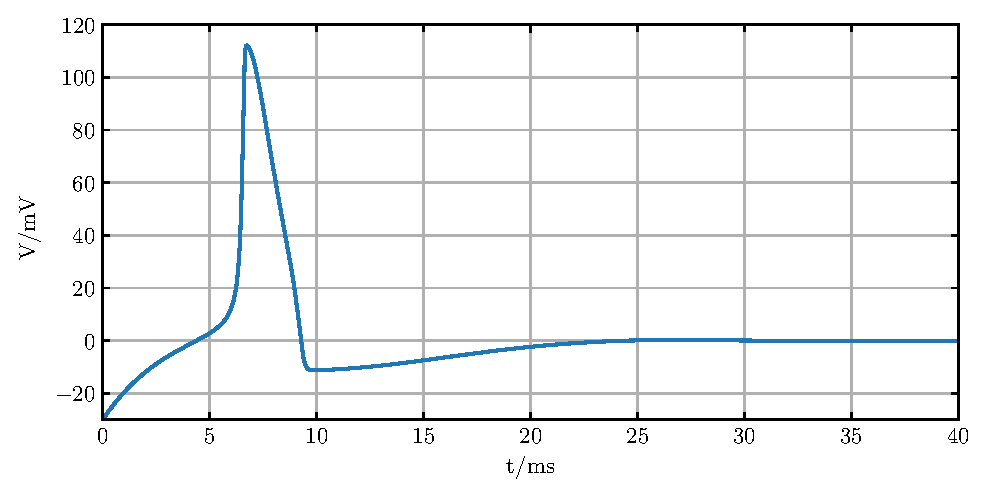
\includegraphics[width=.75\textwidth]{hh52-40ms}
    \caption{H\&H for \SI{40}{\milli\second}; note the hyperpolarization}
    \label{fig:hh2}
\end{figure}

Another interesting effect can be observed when adding an additional source
current density to equation \eqref{eq:cap}, \ie:
\begin{equation*}
    C\,\dv{V}{t}=-\sum_{s}I_{s} + I_{\mathrm{source}}
\end{equation*}
which causes the membrane potential to depolarize again after repolarization
with a constant rate as depicted in \figref{fig:hh3}. Note, that the cell is
firing with a fixed minimal rate given by $I_{\mathrm{source}}$ (All-or-None
principle).

\begin{figure}[h]
    \centering
    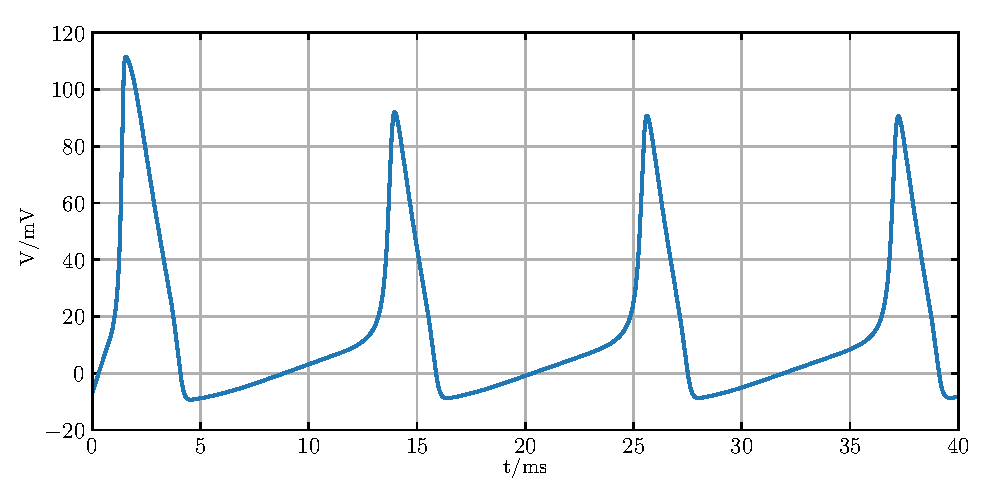
\includegraphics[width=.75\textwidth]{hh52-40ms-10nA}
    \caption{H\&H with
        $I_{\mathrm{source}}=\SI{10}{\ampere\per\metre\squared}$}
    \label{fig:hh3}
\end{figure}


\subsection{Aliev \& Panfilov}
\emph{Note:} The action potential $V$ in this model takes values in $(0,1)$ and
needs to be rescaled according to
$V_{\mathrm{phys}}/\si{\milli\volt}=100\,V-80$. The simulation time $t$ is related
to the physical time via $t_{\mathrm{phys}}/\si{\milli\second}=12.9\,t$.

\vspace{\baselineskip}
The integration was performed for \SI{60}{\stu} (simulationt time units,
\ie~$t_{\mathrm{phys}}=\SI{774}{\milli\second}$) with a time step of
$\Delta{t}=\SI{.01}{\stu}$, resulting in 6000 integration steps and an initial
excitement of the potential to $V_0=\SI{.2}{svu}$ (simulation voltage units,
\ie~$V_{\mathrm{phys},0}=\SI{-60}{\milli\volt}$).

Upon an excitement which surpasses some threshold, the action potential quickly
raises up to its maximal value and decreases rather weakly at first, thus
forming a plateau. The relaxation variable begins raising, too, slowly at
first, but gradually growing faster until it steeply reaches its peak, which
pulls the action potential back to its resting value.

\begin{figure}[h]
    \centering
    \begin{subfigure}[b]{.45\textwidth}
        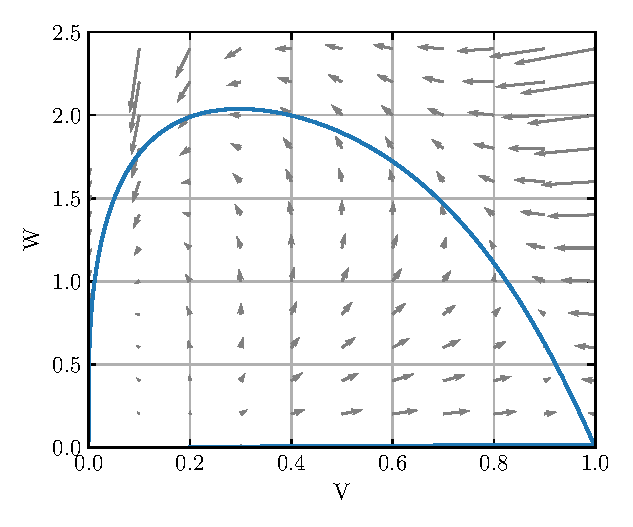
\includegraphics[width=\textwidth]{alpha-phase}
        \vspace{-\baselineskip}
        \caption{Phase plot of the system, shows the characteristic connection
        of the two variables (unscaled)}
        \label{fig:alphaphase}
    \end{subfigure}
    ~
    \begin{subfigure}[b]{.45\textwidth}
        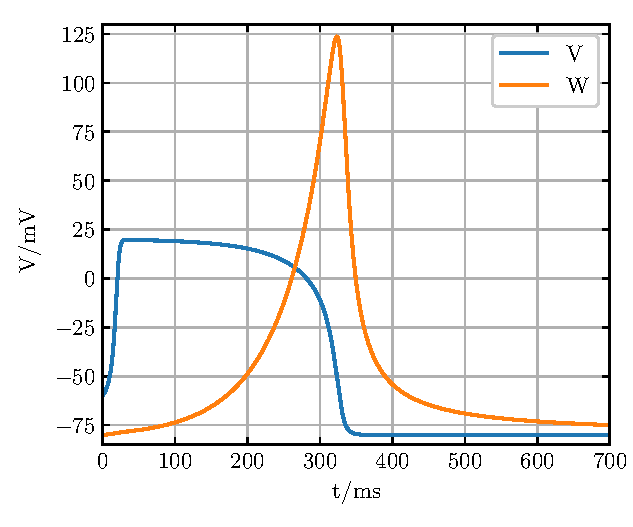
\includegraphics[width=\textwidth]{alpha-dynamics}
        \vspace{-\baselineskip}
        \caption{Temporal evolution of the two variables (physically rescaled)}
        \label{fig:alphadyn}
    \end{subfigure}
    \caption{Results of integrating the A\&P model}
    \label{fig:alpha1}
\end{figure}

The model dynamics are governed by a set of five parameters $a, k, \epsilon_0,
\mu_1\text{ and }\mu_2$. They are phenomenological in their nature and therefor
difficult to interpret. A quick study which varies each parameter while holding
the others constant is found in the appendix (\ref{app:ap-params}).


\subsection{Fenton et al}
\emph{Note:} In this model the action potential also takes values in $(0,1)$
and needs to be rescaled with $V_{\mathrm{phys}}/\si{\milli\volt}=100\,V-80$;
however, the simulation time closely resembles the physical time.

\vspace{\baselineskip}
The integration was performed for \SI{400}{\milli\second} using a time step
$\Delta{t}=\SI{.1}{\milli\second}$ (resulting in 4000 integration steps) and
an initial excitement of the potential $V_0=\SI{.3}{\svu}$
(\ie~$V_{\mathrm{phys}}=\SI{-50}{\milli\volt}$).

The resulting action potential qualitatively resembles the result from the
Aliev-Panfilov model, with the difference that the peak does not start
decreasing right after the excitement but rather shows a slight bump in the
plateau.
Just like the Hodgkin-Huxley model, the Fenton model is  based on an ionic
description, which allows to comprehend the action potential dynamics based on
underlying gate and current processes.

\begin{figure}[h]
    \centering
    \begin{subfigure}[b]{.3\textwidth}
        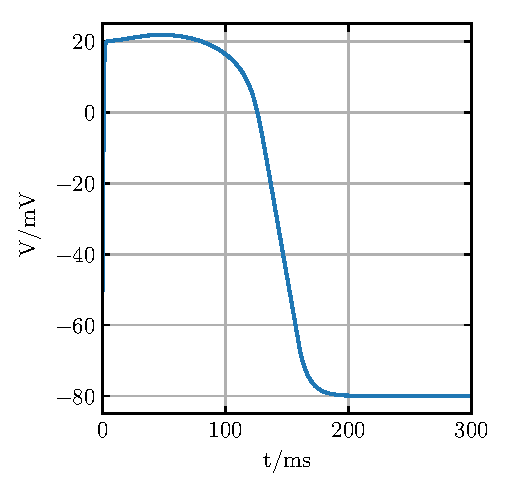
\includegraphics[width=\textwidth]{fenton-single-cell-V}
        \vspace{-\baselineskip}
        \caption{Potential}
        \label{fig:fenton1-V}
    \end{subfigure}
    \vspace{\baselineskip}
    \begin{subfigure}[b]{.3\textwidth}
        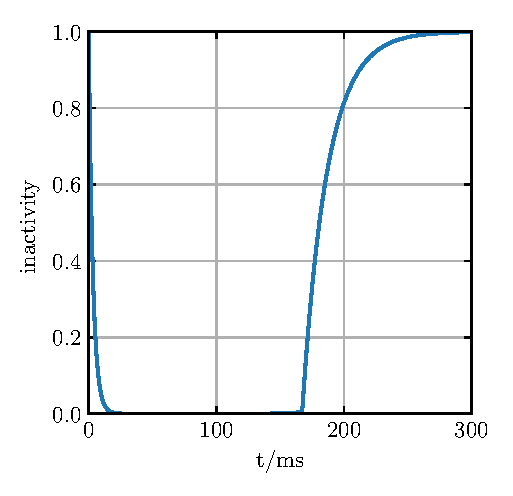
\includegraphics[width=\textwidth]{fenton-single-cell-gate-v}
        \vspace{-\baselineskip}
        \caption{Inactivation gate v}
        \label{fig:fenton1-v}
    \end{subfigure}
    \begin{subfigure}[b]{.3\textwidth}
        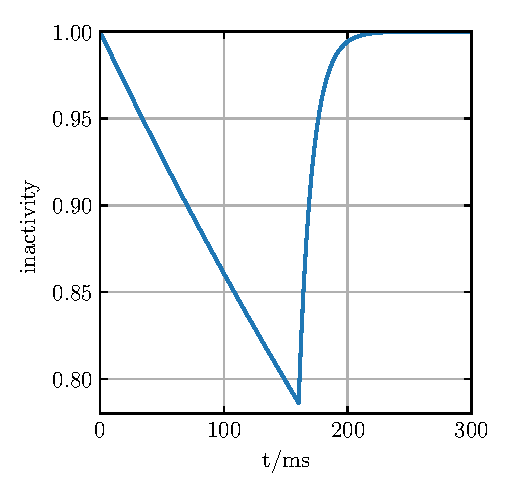
\includegraphics[width=\textwidth]{fenton-single-cell-gate-w}
        \vspace{-\baselineskip}
        \caption{Inactivation gate w}
        \label{fig:fenton1-w}
    \end{subfigure}
    % \vspace{\baselineskip}
    \begin{subfigure}[b]{.3\textwidth}
        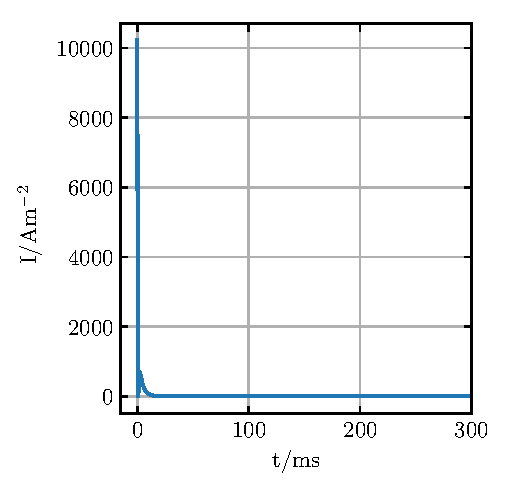
\includegraphics[width=\textwidth]{fenton-single-cell-Ifi}
        \vspace{-\baselineskip}
        \caption{fast inward current}
        \label{fig:fenton1-Ifi}
    \end{subfigure}
    \begin{subfigure}[b]{.3\textwidth}
        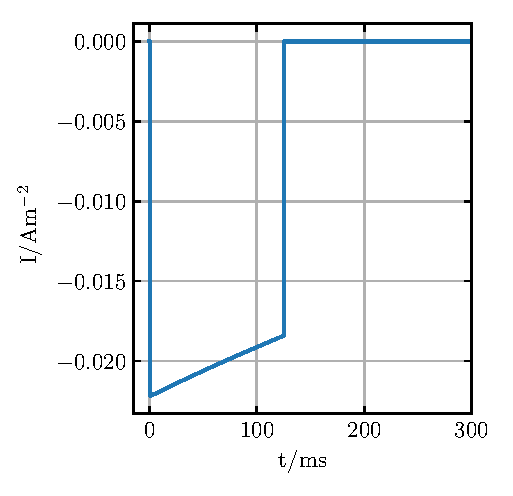
\includegraphics[width=\textwidth]{fenton-single-cell-Isi}
        \vspace{-\baselineskip}
        \caption{slow inward current}
        \label{fig:fenton1-Isi}
    \end{subfigure}
    \begin{subfigure}[b]{.3\textwidth}
        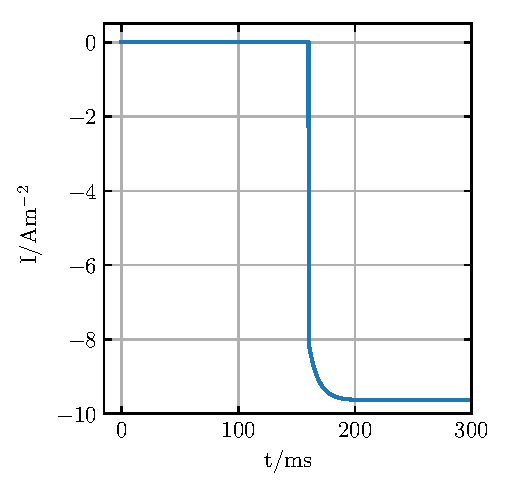
\includegraphics[width=\textwidth]{fenton-single-cell-Iso}
        \vspace{-\baselineskip}
        \caption{slow outward current}
        \label{fig:fenton1-Iso}
    \end{subfigure}
    \caption{Results of integrating the Fenton model}
    \label{fig:fenton1}
\end{figure}

Here are a few things to note:
\begin{itemize}
    \item the gate variables are \emph{inactivation gates}, \ie~1 means fully
        closed, while 0 means fully opened
    \item while the fast inactivation gate $v$ opens completely upon
        excitement and then returns into its closed state, the
        slow inactivation gate $w$ does not open completely (only ca.~21\%)
        before closing again rather quickly.
    \item the currents are modeled with Heaviside-functions in order to be
        activated at once when the potential surpasses a certain threshold
        (given by the parameters $V_c$ and $V_v$); this causes the sudden jumps
        in the plots of the current densities
\end{itemize}


% vim: set ff=unix tw=79 sw=4 ts=4 et ic ai :


\section{Continuous Spatial Dynamics}
The spatial tissue simulations discussed in this section are based on a
continuous approximation of the tissue, which in reality is composed of
discrete cells. The mathematical approach was introduced in section
\ref{sec:contdescr}. In practice -- regardless of the specific model used --
one adds a diffusion term to the ODE describing the temporal evolution of the
membrane potential and obtains a parabolic PDE:
\begin{equation*}
    \pdv{V}{t}=G(V)\longrightarrow\pdv{V}{t}=\eta\,\nabla^2{V}+G(V)
\end{equation*}

In this case the -- usually anisotropic -- diffusivity is given by the scalar
coefficient $\eta$, which was set to $\eta=0.3$ in all cases presented below.
Additionally, the time step is computed in each case to fulfill the CFL
condition:
\begin{equation*}
    \Delta{t}<\frac{(\Delta{x})^2}{2\,\eta}
\end{equation*}


\subsection{On a one-dimensional domain}
\label{sec:1d}
The simulation was performed using the Aliev-Panfilov model. For the
calculations two one-dimensional arrays were used, representing the values of the membrane
potential and the relaxation variable along a discretized line, the length of
which has been varied throughout the simulations while holding the grid
spacing constant at $\Delta{x}=0.2$.

At the beginning von-Neumann boundary conditions were imposed and the first
value of the potential array was set to one. Then at each time step both arrays
were updated using a simple Euler scheme according to
\begin{align*}
    \pdv{V}{t}&=\eta\,\pdv[2]{V}{x}+G_{V}(V, W) \\
    \pdv{W}{t}&=G_{W}(V, W)
\end{align*}
where $G_V$ and $G_W$ are the right hand sides in \eqref{eq:ap_pot} and
\eqref{eq:ap_relax} respectively.

After sufficient steps for the peak of the action potential to develop, the
von-Neumann boundary conditions are replaced by periodic boundary
conditions, which mimics a one-dimensional conducting ring along which an
action potential travels.

When performing the simulation for different lengths, one finds several
quantities of interest:
\begin{description}
    \item[Base Cycle Length] \emph{BCL}, the time for the peak to travel along
        the line once (the time between two peaks, the period)
    \item[Conduction Velocity] \emph{CV}, Velocity of the peak (length of line
        divided by BCL)
    \item[Action Potential Duration] \emph{APD}, time between upstroke and
        downstroke
    \item[Rise Time] duration of upstroke
    \item[Maximal Peak Height]
\end{description}

These quantities were measured by monitoring a fixed point on the domain and
checking at each time step whether the potential crossed either a low or a high
threshold (5\% and 95\% of the maximal potential respectively).
The length of the domain was varied between 25 and 200 and for each value 10
measurements were recorded by letting the peak pass through the domain 10 times after
reaching a stable shape. Then average and standard deviation were computed and
plotted (see \figref{fig:alpha2}).
For lengths below 25 the pulse can not sustain itself with the used parameters.

\begin{figure}[h]
    \centering
    \begin{subfigure}[b]{.3\textwidth}
        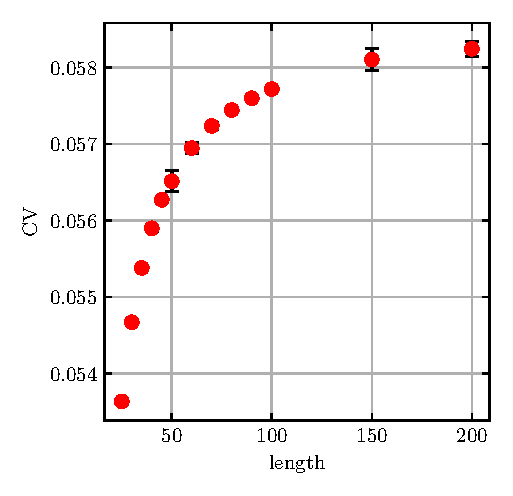
\includegraphics[width=\textwidth]{alpha-measurements-cv}
        \vspace{-\baselineskip}
        \caption{conduction velocity}
        \label{fig:alpha-measure-cv}
    \end{subfigure}
    \vspace{\baselineskip}
    ~
    \begin{subfigure}[b]{.3\textwidth}
        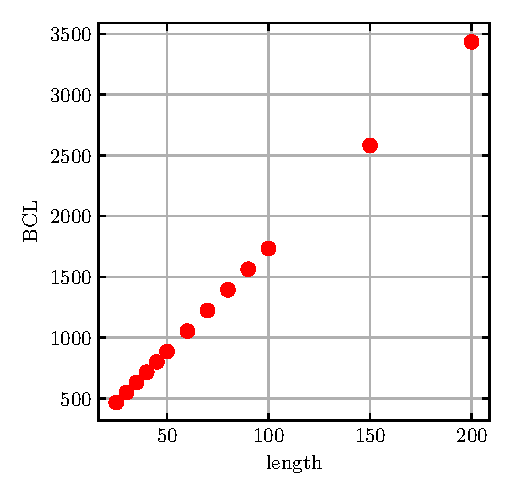
\includegraphics[width=\textwidth]{alpha-measurements-bcl}
        \vspace{-\baselineskip}
        \caption{base cycle length}
        \label{fig:alpha-measure-bcl}
    \end{subfigure}
    ~
    \begin{subfigure}[b]{.3\textwidth}
        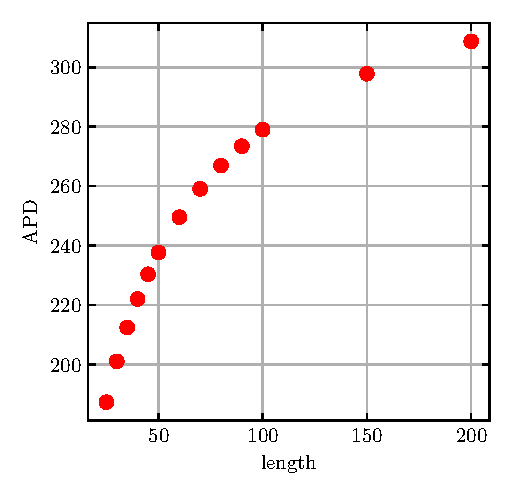
\includegraphics[width=\textwidth]{alpha-measurements-apd}
        \vspace{-\baselineskip}
        \caption{action potential duration}
        \label{fig:alpha-measure-apd}
    \end{subfigure}
    \begin{subfigure}[b]{.3\textwidth}
        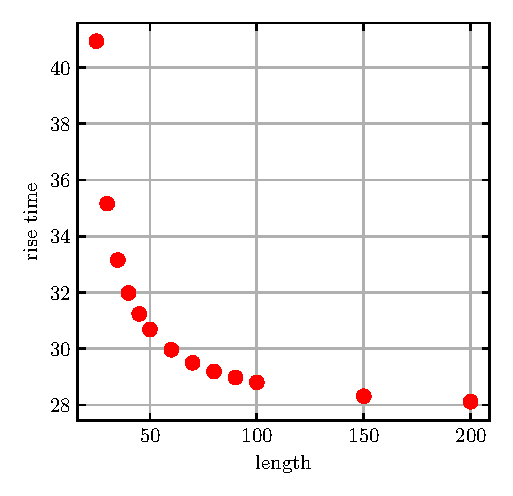
\includegraphics[width=\textwidth]{alpha-measurements-rt}
        \vspace{-\baselineskip}
        \caption{rise time}
        \label{fig:alpha-measure-rt}
    \end{subfigure}
    ~
    \begin{subfigure}[b]{.3\textwidth}
        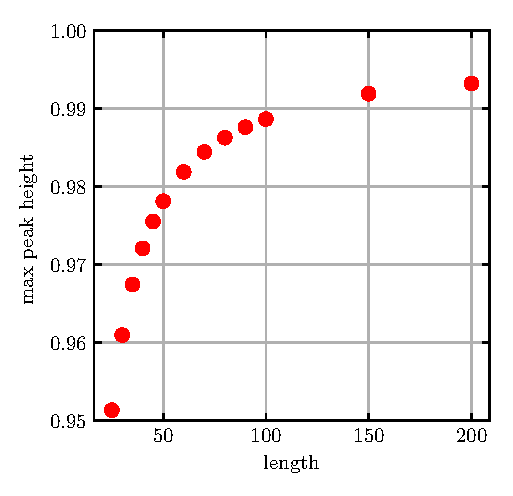
\includegraphics[width=\textwidth]{alpha-measurements-vmax}
        \vspace{-\baselineskip}
        \caption{max peak height}
        \label{fig:alpha-measure-vmax}
    \end{subfigure}
    \caption{All measured quantities plotted against the domain length}
    \label{fig:alpha2}
\end{figure}

Of course, the BCL increases linearly with the maximal length.  The CV and
maximal peak height have smaller values for small lengths. With longer lengths
those values first increase strongly in value and then seem to strive
asymptotically against some upper limit (CV 0.0582, max peak: 0.9931).  The APD
seems to behave similarly, but to verify its asymptotic character, a closer
investigation is required.  The rise time is maximal for small lengths, then
falls and goes towards some lower limit. One can conclude therefrom, that the
action potentials rising edge is the most shallow for high rates and gets
steeper for lower rates.

Concerning the theoretical estimated relationship between CV and rise time
\begin{equation}
    CV\approx\sqrt{\frac{\eta}{2\tau}}(1-2\alpha)
    \label{eq:cvrt}
\end{equation}
the measured values were plotted in \figref{fig:alpha-cv-rt} together with the
curve given by \eqref{eq:cvrt} (where $\alpha=0.17$ was obtained by fitting the
measured data to the formula using a non-linear least squared method; this is
justified, since $\alpha$ acts only as an offset).

\begin{figure}[h]
    \centering
    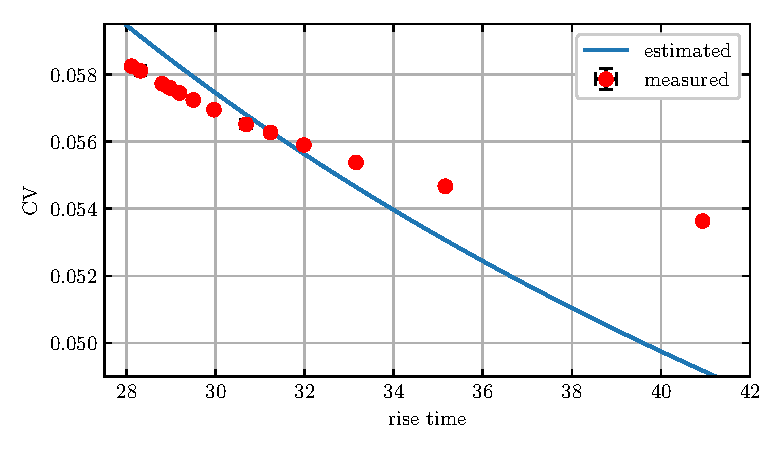
\includegraphics[width=.65\textwidth]{alpha-measurements-cv-rt}
    \caption{comparison of measurement and estimate}
    \label{fig:alpha-cv-rt}
\end{figure}

In order to (naively) quantize this result, both curves were approximated as
linear and a linear regression was computed (see table~\ref{tab:linreg}).
\begin{table}[h]
    \centering
    \begin{tabular}{l | c c}
        \toprule
        & {slope} & {$r^2$-value} \\
        \midrule
        \textbf{measured} & \num{-3.7e-4} & 0.92 \\
        \textbf{estimated} & \num{-7.7e-4} & 0.99 \\
        \bottomrule
    \end{tabular}
    \caption{Results of linear regression}
    \label{tab:linreg}
\end{table}
The relative error of the slopes is ca.~48\%.


\subsection{On a two-dimensional domain}
\label{sec:2d}
The setups described below were simulated with the Aliev-Panfilov model and
with the Fenton model. However hereafter only the results from the Fenton model
are presented, since while exhibiting the same phenomena as the
first-mentioned, it also shows some additional interesting features.

The Fenton simulation is based on three two-dimensional arrays holding the
spatially resolved values of the membrane potential and the two inactivation
gates. These arrays are update each time step with an Euler scheme according to
\begin{align*}
    \pdv{V}{t}&=\eta\,\nabla^2{V}+G_{V}(V, v, w) \\
    \pdv{v}{t}&=G_{v}(V, v, w) \\
    \pdv{w}{t}&=G_{w}(V, v, w)
\end{align*}
where $G_V$, $G_v$ and $G_w$ are the right hand sides in \eqref{eq:cap},
\eqref{eq:v} and \eqref{eq:w} respectively.

All of the following setups used grid steps $\Delta{x}=\Delta{y}=1$. Varying
this parameter corresponds simply to a rescaling of the system.


\subsubsection{Channel}
\label{sec:channel}
One considers a $64\times256$ grid with Dirichlet boundary conditions imposed
along the long side (\ie~the x-direction) and periodic boundary conditions
along the short side (\ie~the y-direction).

For the initial values of $V$ and $w$ the same narrow stripe (20 grid points
wide) and for $v$ a stripe of same width but shifted 10 grid points in positive
x-direction were set to 1.

Running the simulation, an action potential quickly develps and repeatedly
passes through the domain, which mimics a constant rate of pulses. Because of
the Dirichlet conditions the action potential on the edges is pulled to zero,
causing some kind of tail (see \figref{fig:pulse}).

\begin{figure}[h]
    \centering
    
\includegraphics[width=.75\textwidth]{fenton-cont-pulse}
    \caption{Pulse in channel setup}
    \label{fig:pulse}
\end{figure}


\subsubsection{Spiral Excitation}
\label{sec:spiral1}
Now one considers a $128\times512$ grid with von-Neumann boundary conditions
imposed on all sides. The initial conditions to generate the first pulse are
the same as described above. Because of the boundary conditions, the pulse is
not damped on the edges and passes through the domain only once.

Now a small area of $10\times10$ grid points right in the middle of the domain
has its membrane potential set to 1. In the absence of any prior excitation
this simply produces a circular pulse running away in all directions. But if
this perturbation happens in the wake of a preceding action potential an
interaction with the relaxation variables - which have not yet fully returned
to their rest values - takes place: Either the perturbation is suppressed right
away, or it is pushed backwards growing into the shape of an expanding
croissant whose edges are running forward until they meet in the
center. Upon this meeting the croissant becomes a pretzel which runs away in a
circular fashion and the then slightly inwards turned edges generate a new
croissant-shaped pulse which undergoes the same process.

\begin{figure}[h]
    \centering
    \begin{subfigure}[b]{.45\textwidth}
        
\includegraphics[width=\textwidth]{spiral-80}
        \vspace{-\baselineskip}
        \caption{2400 steps}
    \end{subfigure}
    \begin{subfigure}[b]{.45\textwidth}
        
\includegraphics[width=\textwidth]{spiral-81}
        \vspace{-\baselineskip}
        \caption{2430 steps}
    \end{subfigure}
    \begin{subfigure}[b]{.45\textwidth}
        
\includegraphics[width=\textwidth]{spiral-84}
        \vspace{-\baselineskip}
        \caption{2520 steps}
    \end{subfigure}
    \begin{subfigure}[b]{.45\textwidth}
        
\includegraphics[width=\textwidth]{spiral-87}
        \vspace{-\baselineskip}
        \caption{2610 steps}
    \end{subfigure}
    \begin{subfigure}[b]{.45\textwidth}
        
\includegraphics[width=\textwidth]{spiral-100}
        \vspace{-\baselineskip}
        \caption{3000 steps}
    \end{subfigure}
    \begin{subfigure}[b]{.45\textwidth}
        
\includegraphics[width=\textwidth]{spiral-110}
        \vspace{-\baselineskip}
        \caption{3300 steps}
    \end{subfigure}
    \begin{subfigure}[b]{.45\textwidth}
        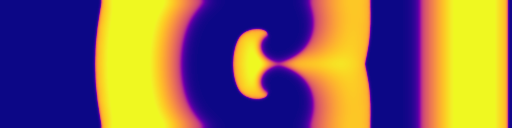
\includegraphics[width=\textwidth]{spiral-120}
        \vspace{-\baselineskip}
        \caption{3600 steps}
    \end{subfigure}
    \begin{subfigure}[b]{.45\textwidth}
        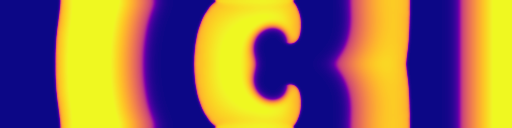
\includegraphics[width=\textwidth]{spiral-130}
        \vspace{-\baselineskip}
        \caption{3900 steps}
    \end{subfigure}
    \caption{Image series of spiral excitation due to well-timed perturbation}
    \label{fig:spiral}
\end{figure}

For the given setup, the sweet spot in insert this perturbation lies around
2430 integration steps (see \figref{fig:spiral}).

While with the Fenton model each succeeding spiral is slightly damped causing
the process to be extinguished completely after a finite number of iterations,
the spirals generated with the Aliev-Panfilov model do not seem to exhibit such
kind of behaviour and instead go on indefinitely.


\subsubsection{Spiral Wave and Breakup}
\label{sec:spiral2}
Finally one considers a $256\times512$ grid with von-Neumann boundary
conditions on all sites. The initial conditions are given by a stripe of
excited membrane potential which only reaches into the domain by some extend,
\ie~it has a loose end.

When performing the simulation, the main part of the initial stripe develops
into a pulse like seen before, but the loose end turns away growing into a
spiral and eventually hits its own wake. When the tip reaches not yet fully
repolarized tissue, it fails to continue propagating normally and instead
breaks up (in the Fenton model this is due to the interaction of the action
potential of the tip with the inactivation gates in the wake). This process
starts to successively generate new spirals. It amplifies itself, soon causing
multiple spirals to be present at once, which spread out until the whole domain
is disruptively filled with small and rather fast moving spirals (see
\figref{fig:breakup}).

\begin{figure}[h]
    \centering
    \begin{subfigure}[b]{.3\textwidth}
        
\includegraphics[width=\textwidth]{breakup-1}
        \vspace{-\baselineskip}
        \caption{50 steps}
    \end{subfigure}
    \begin{subfigure}[b]{.3\textwidth}
        
\includegraphics[width=\textwidth]{breakup-6}
        \vspace{-\baselineskip}
        \caption{300 steps}
    \end{subfigure}
    \begin{subfigure}[b]{.3\textwidth}
        
\includegraphics[width=\textwidth]{breakup-10}
        \vspace{-\baselineskip}
        \caption{500 steps}
    \end{subfigure}
    \begin{subfigure}[b]{.3\textwidth}
        
\includegraphics[width=\textwidth]{breakup-20}
        \vspace{-\baselineskip}
        \caption{1000 steps}
    \end{subfigure}
    \begin{subfigure}[b]{.3\textwidth}
        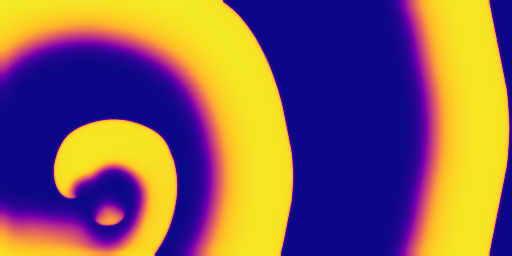
\includegraphics[width=\textwidth]{breakup-40}
        \vspace{-\baselineskip}
        \caption{2000 steps}
    \end{subfigure}
    \begin{subfigure}[b]{.3\textwidth}
        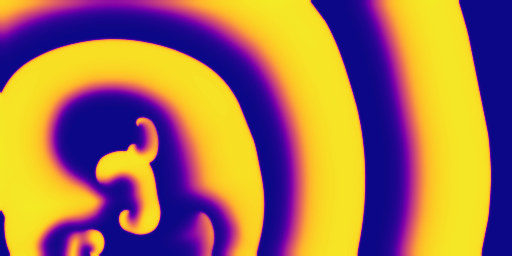
\includegraphics[width=\textwidth]{breakup-60}
        \vspace{-\baselineskip}
        \caption{3000 steps}
    \end{subfigure}
    \begin{subfigure}[b]{.3\textwidth}
        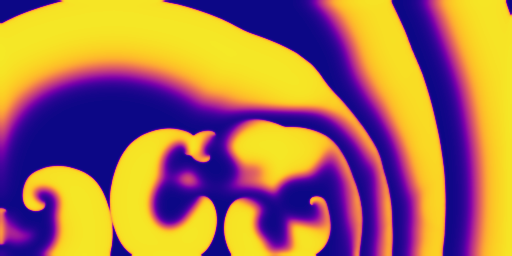
\includegraphics[width=\textwidth]{breakup-90}
        \vspace{-\baselineskip}
        \caption{4500 steps}
    \end{subfigure}
    \begin{subfigure}[b]{.3\textwidth}
        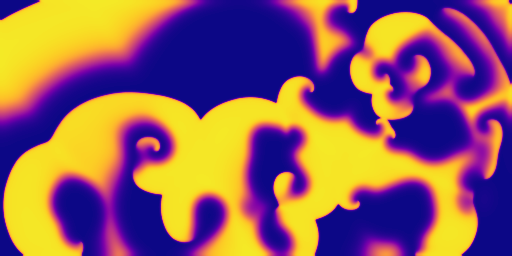
\includegraphics[width=\textwidth]{breakup-120}
        \vspace{-\baselineskip}
        \caption{6000 steps}
    \end{subfigure}
    \begin{subfigure}[b]{.3\textwidth}
        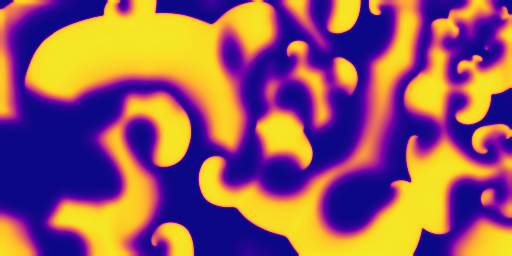
\includegraphics[width=\textwidth]{breakup-150}
        \vspace{-\baselineskip}
        \caption{7500 steps}
    \end{subfigure}
    \caption{Image series of spiral wave breakup due to tip-wake interaction}
    \label{fig:breakup}
\end{figure}

With the Aliev-Panfilov model the aforementioned initial conditions generate
an ever-growing spiral without any disruptive behaviour.


% vim: set ff=unix tw=79 sw=4 ts=4 et ic ai :


\section{Physiological Interpretation}
\label{sec:phys}
\subsection{One-dimensional ring}
The one-dimensional ring described in section~\ref{sec:1d} can be interpreted
as a conducting fibre of the hearts conduction system, through which a constant
rate of action potentials passes. This rate can be varied by varying the length
of the ring. While this approach seems rather simplistic, it can be used to
understand the effects of tachycardia (\ie~abnormal high heart rates) on the
characteristics of single action potentials: the peaks are more shallow (longer
rise time), do not reach their full height, have a shorter duration and are
being conducted somewhat slower.

Such deviations from the regular behaviour can express itself as arrhythmia and
have a significant impact on the well-being of the affected person.


\subsection{Channel}
The situation depicted in section~\ref{sec:channel} of a confined channel could
be used to describe a bundle of cells belonging to the electrical conducting
system of the heart, which transmit action potentials at a constant rate to
some target tissue area, in order to trigger its contraction.

While with the default configuration this mimics a properly working propagation
of action potentials, one can also observe above described phenomena when
shortening the length of the domain.


\subsection{Spiral waves}
In a healthy heart the action potential meant to trigger contraction is
propagating homogeneously through the tissue. If now due to some pathological
condition some regions in the cardiac tissue have different electrical
conductivities or do not conduct at all (scar tissue), the action potential
might travel around these obstacles eventually hitting its own wake and causing
local depolarization deviating from the beat given by the SA node.
Such phenomena are known as \emph{re-entrant arrhythmia} and can cause ventricular tachycardia
or atrial flutter and might develop into ventricular or atrial fibrillation.
The only way to stop (the otherwise fatal) ventricular fibrillation is to
apply a high energy electrically shock to depolarize all (or a
critical mass) of cardiac tissue (defibrillation). When the cells have
repolarized, they can again be governed by the pace given by the SA node.

Those aforementioned phenomena resemble spiral waves, which in reality occur
due to heterogeneity of the tissue. On a simplified homogeneous domain, one can
generate such spiral waves \eg~by delivering a single impulse in the wake of a
propagating action potential wave (see section~\ref{sec:spiral1}) or by
defining an initial wave with a loose end (see section~\ref{sec:spiral2}).
While the spiral waves discussed in section~\ref{sec:spiral1} can be
interpreted as ventricular tachycardia, the disruptive and uncoordinated
dynamics seen in section~\ref{sec:spiral2} resemble ventricular fibrillation
(see also fig.~38 in \cite{Cherry2008}).


\section{Discussion}


% vim: set ff=unix tw=79 sw=4 ts=4 et ic ai :


\appendix
\section{Appendix}
\subsection{Varying the parameters of the Aliev \& Panfilov model}
\label{app:ap-params}

Here is a quick study presented, which varies the parameters of the phenomenological
Aliev-Panfilov model \eqref{eq:ap_eqs} and examines its behaviour:
table~\ref{tab:apparams} gives an overview including a description of the
resulting change and in fig.~\ref{app:apparams} these changes were plotted.

\begin{table}[h]
    \centering
    % {\renewcommand{\arraystretch}{2}%
    \begin{tabular}{C c p{8cm}}
        \toprule
        \text{Name} & Range & Effect \\
        \midrule
        a & \numrange{.1}{.2} &
            \tabitem delay of $V$ and $W$ \\
        & & \tabitem $a=0.2$: both variables are extinguished \\[.6em]
        k & \numrange{4.}{14.} &
            \tabitem scaling strength and slope of $W$ \\
        & & \tabitem the larger $k$, the faster and stronger
            rises $W$ \\[.6em]
        \epsilon_0 & \numrange{1e-5}{1.} &
            \tabitem makes $W$ rise earlier \\
        & & \tabitem maintains the peak's shape \\[.6em]
        \mu_1 & \numrange{.05}{2.} &
        \tabitem makes $W$ rise earlier and steeper \\[.6em]
        \mu_2 & \numrange{.1}{5.} &
        \tabitem delays $W$ and flattens the peak \\[.6em]
        \bottomrule
    \end{tabular}%}
    \caption{Parameter overview}
    \label{tab:apparams}
\end{table}

\begin{figure}[b]
    \centering
    \begin{subfigure}[b]{\textwidth}
        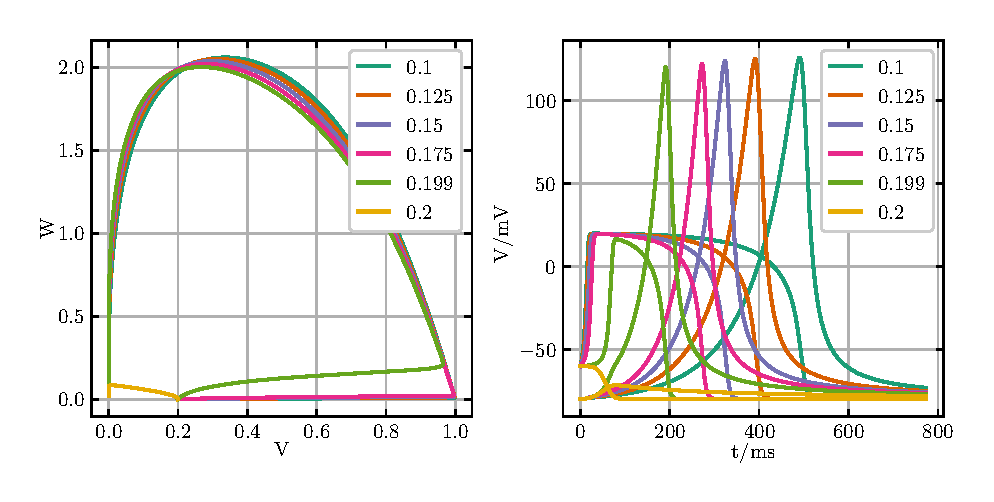
\includegraphics[width=\textwidth]{alpha-params-1}
        \vspace{-2\baselineskip}
        \caption{a}
    \end{subfigure}
    \begin{subfigure}[b]{\textwidth}
        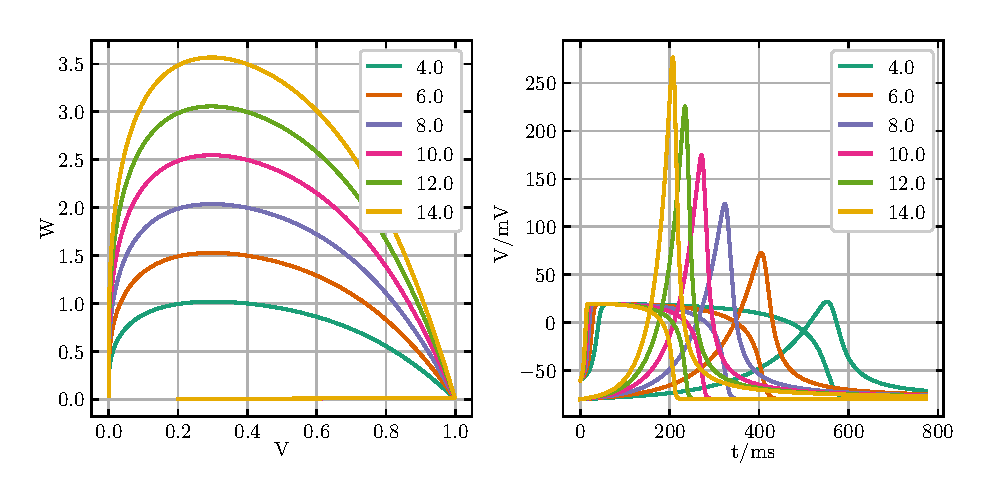
\includegraphics[width=\textwidth]{alpha-params-2}
        \vspace{-2\baselineskip}
        \caption{k}
    \end{subfigure}
    \begin{subfigure}[b]{\textwidth}
        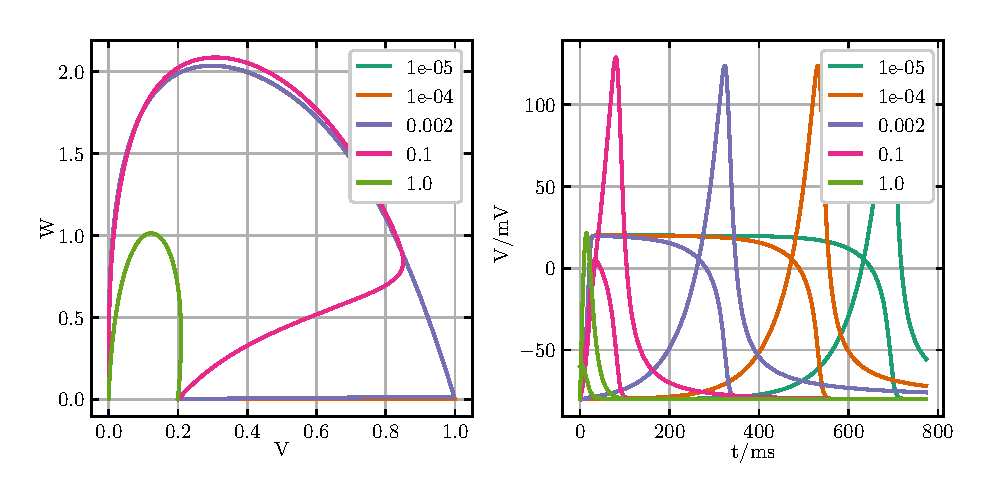
\includegraphics[width=\textwidth]{alpha-params-3}
        \vspace{-2\baselineskip}
        \caption{$\epsilon_0$}
    \end{subfigure}
\end{figure}
\begin{figure}[t]
    \ContinuedFloat
    \centering
    \begin{subfigure}[b]{\textwidth}
        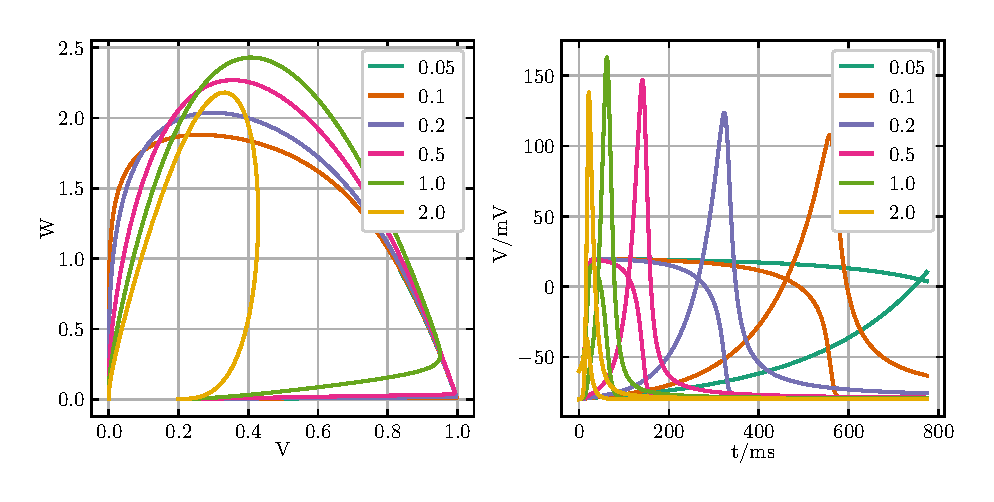
\includegraphics[width=\textwidth]{alpha-params-4}
        \vspace{-2\baselineskip}
        \caption{$\mu_1$}
    \end{subfigure}
    \begin{subfigure}[b]{\textwidth}
        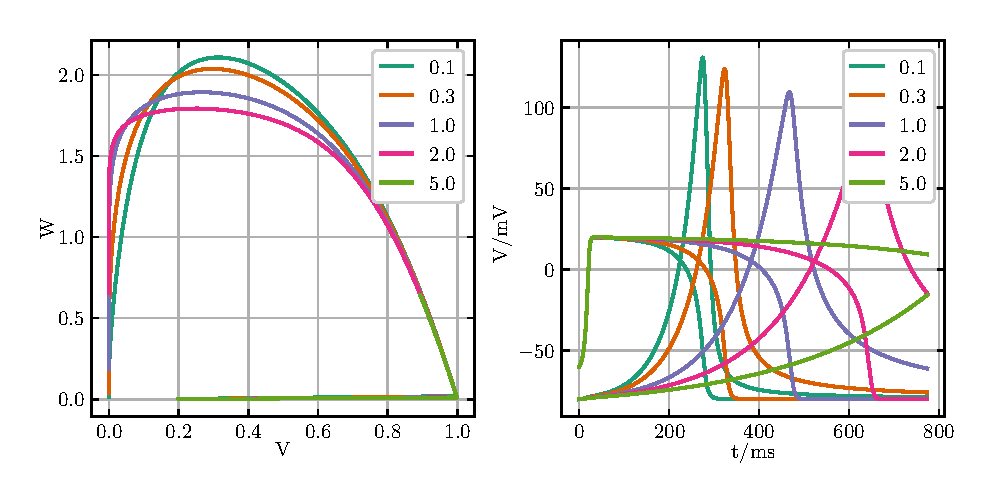
\includegraphics[width=\textwidth]{alpha-params-5}
        \vspace{-2\baselineskip}
        \caption{$\mu_2$}
    \end{subfigure}
    \caption{Plots for varying parameters}
    \label{app:apparams}
\end{figure}


% vim: set ff=unix tw=79 sw=4 ts=4 et ic ai :


\addcontentsline{toc}{section}{Literature}
\nocite{*}
\printbibliography[title=Literature]

\end{document}


% vim: set ff=unix tw=79 sw=4 ts=4 et ic ai :
